\chapter{\chapviiname}
\label{chapter7}
\section*{Overview}
This chapter investigates the phenomenon of unintentional power generation in Dielectric Elastomer Actuator (DEA) devices integrated with Electrical Impedance Tomography (EIT) for pressure mapping applications. While DEAs are primarily designed for actuation, they can inadvertently function as Dielectric Elastomer Generators (DEGs) due to localised mechanical strain during operation. The research explores the mechanisms behind this unintended energy generation, focusing on the changes in capacitance that occur when the DEA is subjected to varying loads. Through experimental simulations, the study quantifies the energy produced, revealing that energy generation can range from 0.2 $\mathrm{\mu}$J to 4 mJ depending on the load conditions. The findings highlight the multi-functionality of DEAs; actuation,sensing, and energy generation, emphasising the need for careful management of energy generation to prevent potential damage to connected circuitry. This work contributes to the understanding of DEA-EIT devices and their applications in soft robotics and simultaneous energy harvesting, suggesting that the energy generated could be harnessed for practical use in various scenarios, including vehicular and foot traffic loads. Future work aims towards harnessing the DEG energy shown in this work and using it to power the portable ERT-circuit in Chapter \ref{chapter5} expanding the range of potential applications.



\section{Introduction} % 1.5 pages
\label{sec:introduction}
% Breifly discuss: the state of the art of DEGs, previous device created, and the intention of this chapter: To elucidate the operation of the DEA-EIT device specifically looking into it's potential function as a DEG.
Dielectric Elastomer Actuators (DEAs) and Dielectric Elastomer Generators (DEGs) share a similar form whereby they both have compliant conductive electrodes either side of a dielectric elastomer (DE) membrane. However, DEGs represent a class of electromechanical devices that harness mechanical strain to generate electrical energy. DEAs and DEGs can often utilise the same soft electroactive area for actuation and power generation, but differ in the connected electronics. These devices exploit the properties of dielectric elastomers, which are soft, flexible materials capable of undergoing significant deformation. This deformation can be utilised to generate electrical power, making DEGs a promising technology for energy harvesting applications. However, DEGs can also arise as an unintended consequence of loading a DEA device.

In typical DEG configurations, the focus has been on uniform, global strain changes within the dielectric elastomer domain. Previous research has concentrated on scenarios where the entire thickness of the DE is reduced as a result of applied strain, leading to energy generation due to global DE deformations \cite{Carpi2015, Savage2012, Koh2009}.

In contrast, this work explores unintentional DEG scenarios that have arisen from the invention of a hybrid actuation and pressure mapping DEA-EIT device. By investigating the effects of localised thickness reduction within the DE caused during a load event during DEA switching, unintended power generation due to the change in the device capacitance is observed.

This localised approach introduces a new dimension to DEG functionality, where strain is not uniformly applied but concentrated in specific areas. This DEA-EIT integration, as discussed in Chapter \ref{chapter7}, allows for precise monitoring and analysis of localised deformations, thereby enhancing understanding potential scenarios where DEG behaviour may occur. In the existing literature, neither the intentional nor unintentional use of a DEA-EIT-like device as a DEG, when subjected to localised loads, has been investigated at the time of writing this work.



\subsection{Background} 
\label{subsec:background}
% Re-iterate in a few sentences how the DEA-EIT sytstem works
Before describing how a dielectric generator arises in DEA-EIT device, it is important to understand the function of a DEA-EIT device first as  described in detail in the previous chapter. A DEA-EIT device can use the same compliant electrodes and dielectric elastomer to function both as an electroactive actuator and pressure mapping sensor. The DEA function consists of applying a high voltage to a bottom electrode leaving the top electrode as the low voltage electrode which performs as the pressure mapping surface. The pressure mapping surface is piezoresistive and uses electrical impedance tomography to map any changes in resistance and hence any loads throughout the electrode surface. 
\begin{figure}[H]
	\centering
	\hspace{1cm}
	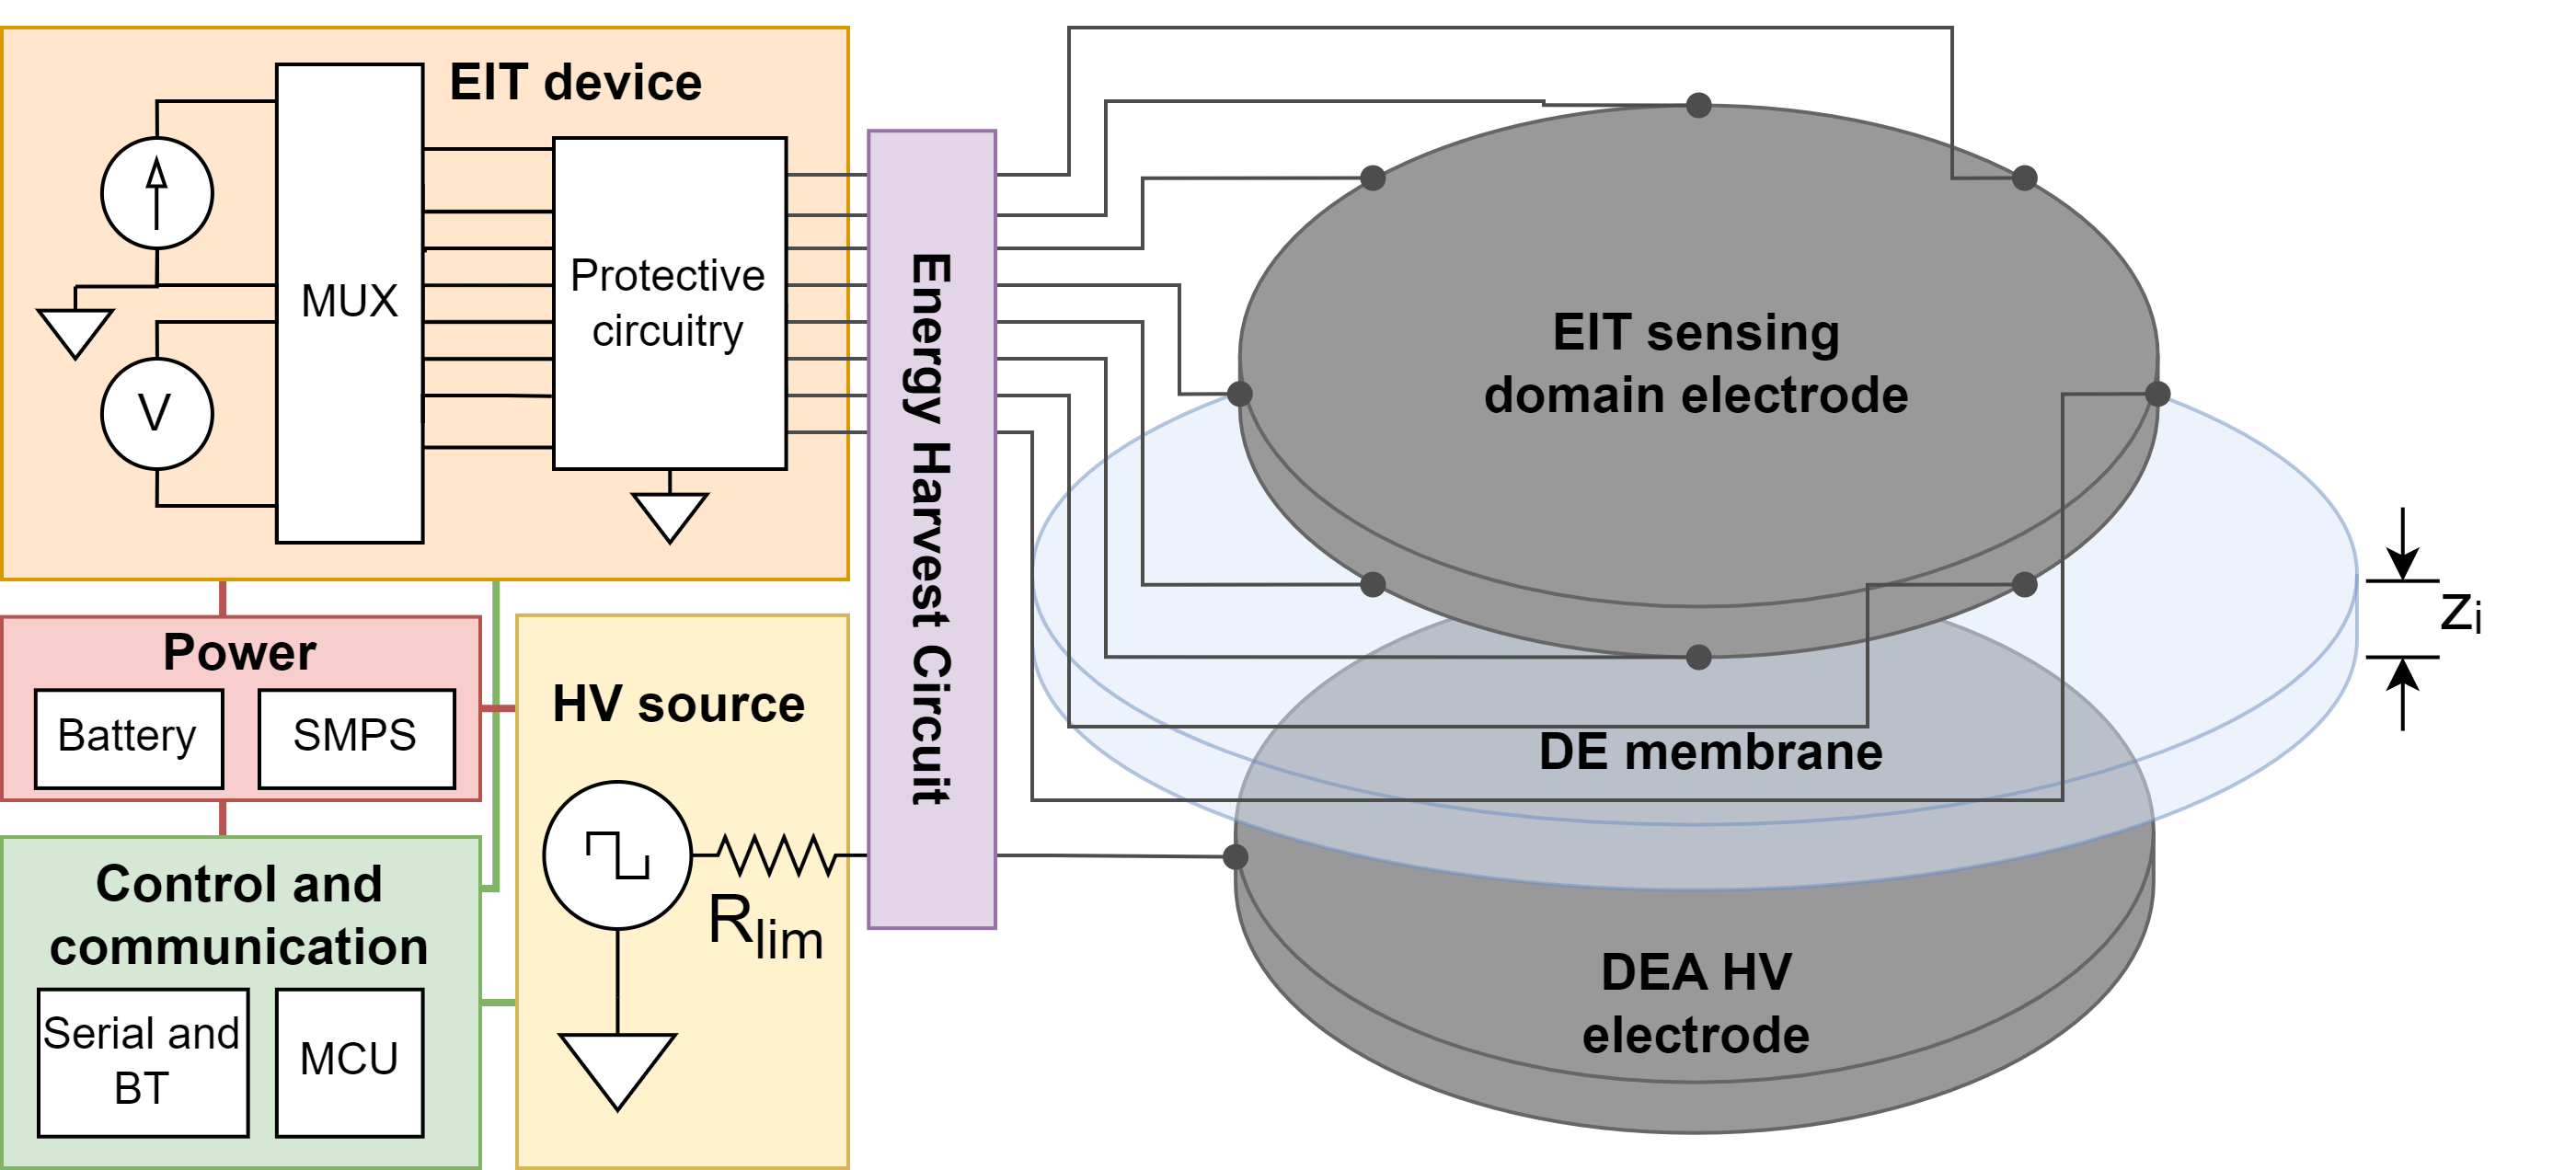
\includegraphics[width=0.8\linewidth]{Figures/DEA-EIT_architecture_v2.png}
	\vspace{0.3cm}
	\caption{Architecture of a DEA-EIT pressure mapping and actuator device with an exploded view of the DEA stack.}
	\label{fig:dea-eit-architecture-w-MCU}
\end{figure}

A DEG may be incidentally be created during simultaneous DEA-EIT operation. This effect will take place when the DEA experiences sufficiently large external strains and DEA voltage switching at specific times. This DEG sequence is shown in Figure \ref{fig:dea_eit_deg} and is explained as five distinct stages.

\begin{figure}[H]
	\centering
	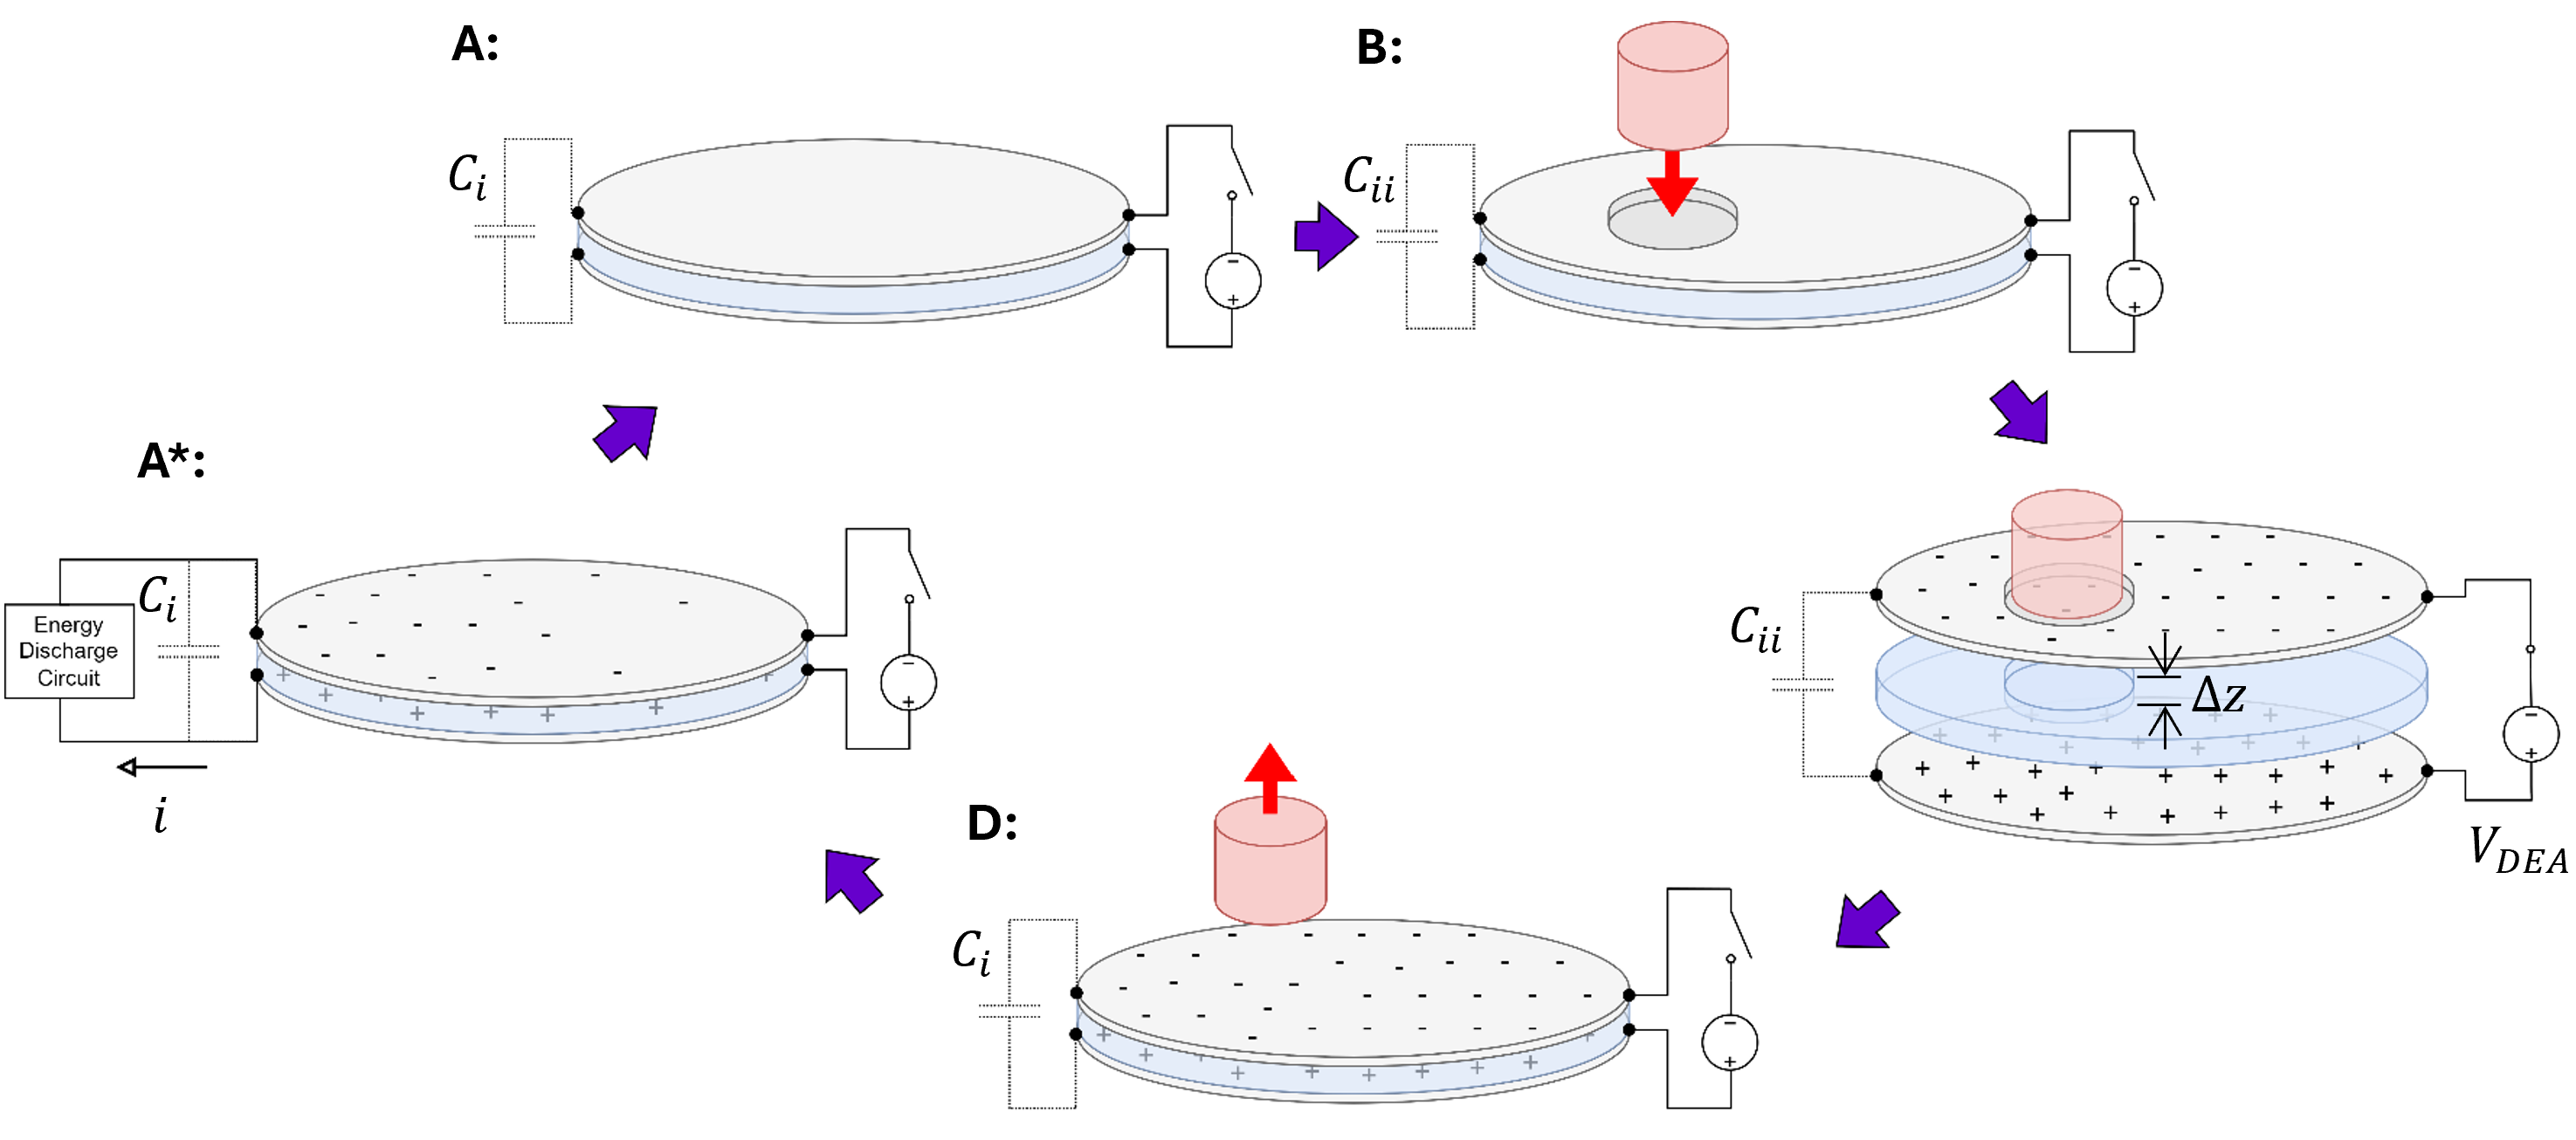
\includegraphics[width = \textwidth]{Figures/DEA-EIT-DEG_sequence_v2.png}
	\vspace{0.2cm}
	\caption{Dielectric elastomer generator scenario sequence with a localised compressive load.}
	\label{fig:dea_eit_deg}
\end{figure}
Where $C_i$ is the initial capacitance of the DEA, $C_{ii}$ is the `primed' capacitance of the DEA, the positive and negative signs, $+$ and $-$, on the compliant electrode represent electrical charge, and the red cylinder represents the load applicator. The typical operation of a DEG consists of the five main stages described below and exemplified in Figure \ref{fig:dea_eit_deg}. Note that the changes in electrostatic force due to loads are ignored.

\textbf{State A}: the DEA has an initial capacitance of $C_i$, is deformation free, and has zero voltage applied across the compliant electrodes.

\textbf{State B}: the DEA is compressed and deformed with a localised change(s) in thickness of the DE, $\Delta z$, increasing the DEA capacitance to $C_{ii}$. Work is done on the DEA by the compressive load storing elastic potential energy in the strained DE.
As derived from Hooke's law the elastic potential energy, $U_{\varepsilon}$ for a material of Young's modulus, $Y$, cross-sectional area, $A_i$, original thickness, $z_i$, and change in thickness, $\Delta z$ is given in Equation \ref{eqn:elastic-energy}. This equation is for a singular body with an even change in thickness across the area, $A_i$, showing the core parameters governing the elastic potential energy.
% Todo: mention that this equation isn't suffice so we use FEM modelling which gives a better representation of the Hookean continuum model but still neglects viscous damping within the material.
\begin{equation}
	U_{\varepsilon} = \frac{YA_i\Delta z^2}{2z_i}
	\label{eqn:elastic-energy}
\end{equation}

\textbf{State C}: An applied voltage, $V_i$, across the compliant electrodes generates electrical charge. The total charge developed, $Q$, is given by Equation \ref{eqn:charge-cap-volt1}.
\begin{equation}
	Q = C_{ii}V_{i}
	\label{eqn:charge-cap-volt1}
\end{equation}
Charging the electrodes gives electrical potential energy to the DEA as it is now a charged capacitor. The electrical potential energy of the DEA is given by Equation \ref{eqn:elec-energy1}.
\begin{equation}
	U_{E(C)} = \frac{1}{2}C_{ii}V_i^2
	\label{eqn:elec-energy1}
\end{equation}

\textbf{State D}: The DEA is unloaded and returns to its original state with capacitance, $C_i$, while maintaining the same charge $Q$ causing the voltage to increase to $V_{ii}$ as shown by Equation \ref{eqn:charge-cap-volt2}.
\begin{equation}
	V_{ii} = \frac{Q}{C_{i}}
	\label{eqn:charge-cap-volt2}
\end{equation}
When the load is released the elastic potential energy, $U_{\varepsilon}$, is used as the DEA returns to a relaxed state. In parallel, the increase in voltage on the DEA increases the electrical potential energy, $U_{E(D)}$ as shown by Equation \ref{eqn:elec-energy2}.
\begin{equation}
	U_{E(D)} = \frac{1}{2}C_{i}V_ii^2
	\label{eqn:elec-energy2}
\end{equation}
Resulting in a gain of electrical potential energy $\Delta U_E$ comprising the difference of $U_{E(C)}$ and $U_{E(D)}$.

\textbf{State A*}: The DEA is discharged into the energy harvesting circuit returning the charge and voltage values across the DEA to zero, returning to State A. 

The unintended power generation discussed may cause issues with the pressure measurement system if switching significantly high DEA voltage source is done during a significant DEA-EIT surface loading event. A significant loading event is one which changes the capacitance of the DEA such that a voltage is generated by the unintended DEG which is high enough to cause potential harm to the EIT driving circuitry. 



\section{Methodology} % 3 pages
\label{sec:method}
% How was the FEM set up? and why?
To confirm the existence of this DEG phenomena in the DEA-EIT device design has undergone a sequence of FEM studies. To determine which compressive loads may give significant capacitance changes that could lead to significant voltage amplification and potentially significant energy generation across DEA electrodes, FEA of a DEA undergoing compressive pressure loading events have been completed. Experimental cases using two different loading areas, as shown in Figure \ref{fig:FEM_DEA-EIT_loading}, with a range of forces were completed. All FEA studies were three dimensional to account for any potential non-symmetric results and variations in fringe effects.
\begin{figure}[H]
	\centering
	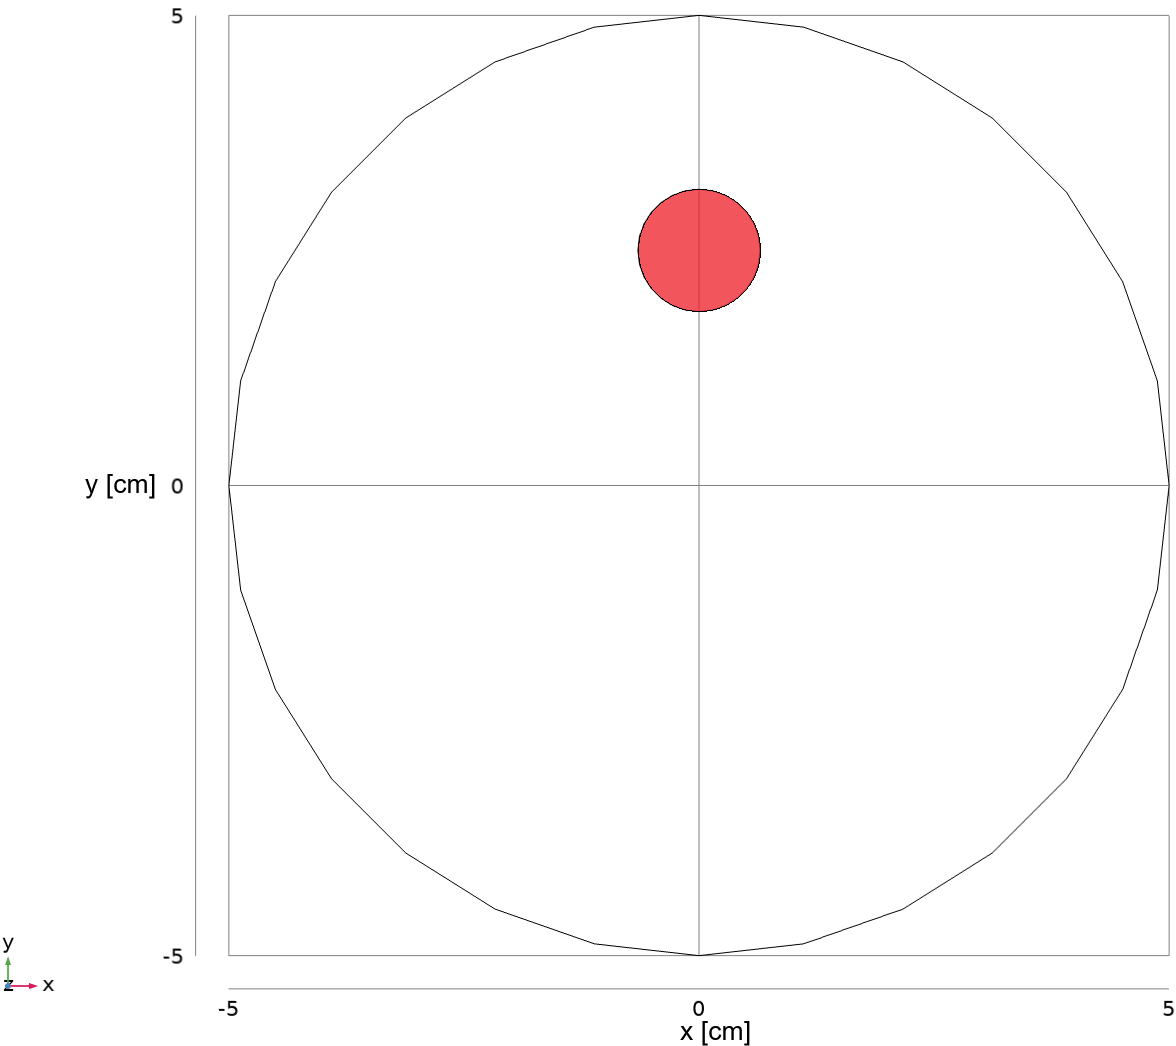
\includegraphics[width=0.45\linewidth]{Figures/d13mm_load_case_comsol2d_red.png} % Todo: change the diagram to elimate the z axis
	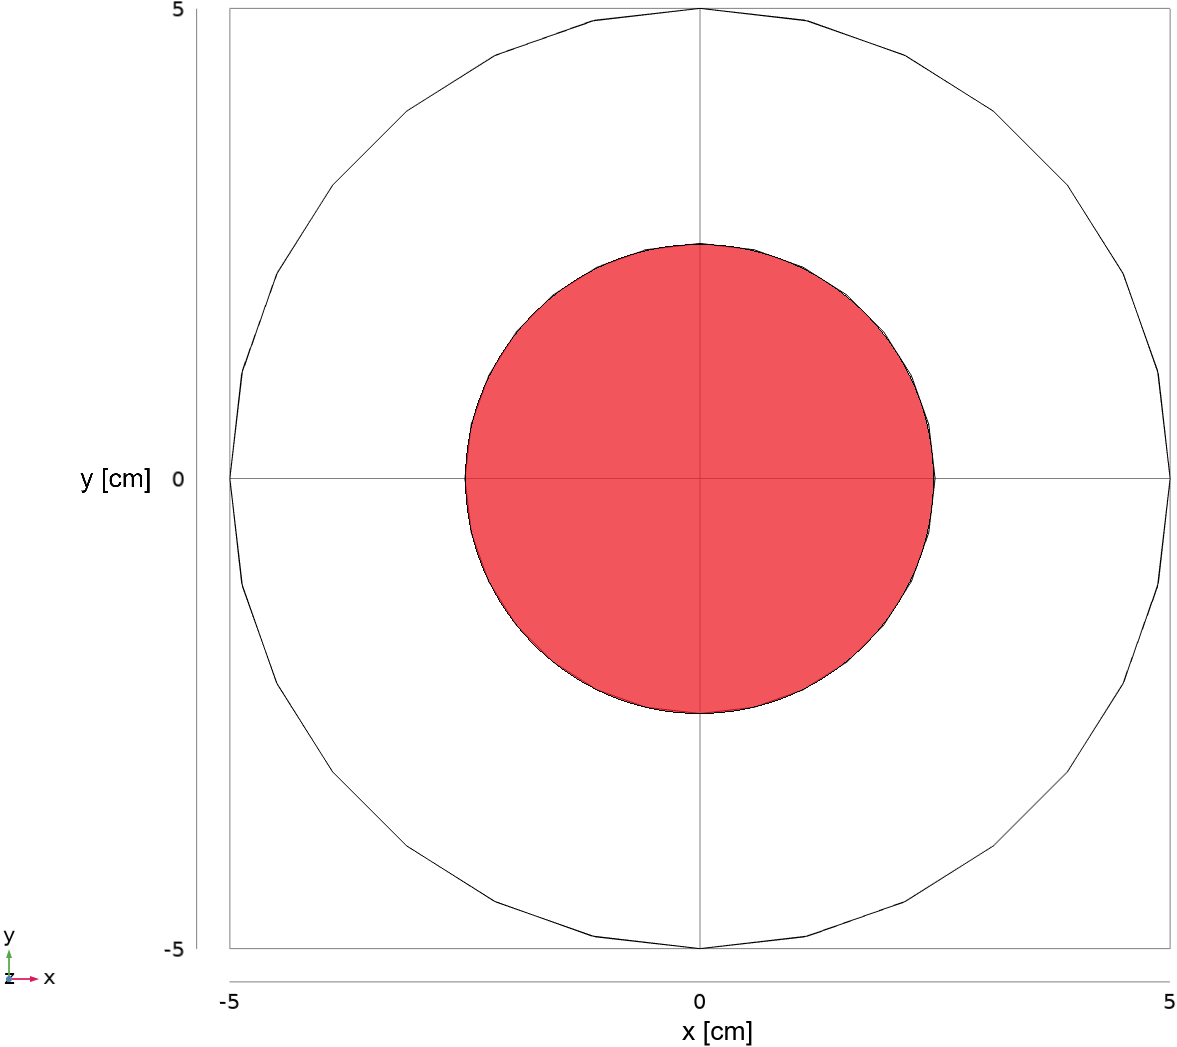
\includegraphics[width=0.45\linewidth]{Figures/d50mm_load_case_comsol2d_red.png} % Todo: change the diagram to elimate the z axis
	% \includegraphics[width=0.3\linewidth]{multi area touch.png}
	\vspace{0.3cm}
	\caption{Loading cases for analysis of capacitance change. Left: 13 mm diameter load. Right: 50 mm diameter load.}
	\label{fig:DEA-EIT_loading}
\end{figure}


\subsection{DEA Load Study}
%% Todo: Describe FEM parameters for DEA loading and FEM tool used!
To obtain a representation of how the DEA structure will deform during a different loading events, a static load FEA study was performed using COMSOL Multiphysics \cite{COMSOL2022} to determine the expected deformation of the DEA and create mesh models. The deformed mesh models were then used for further electrostatic FEM studies to determine the change in capacitance of the DEA structure. A physics controlled mesh was used with a maximum element size of 10 mm and a minimum element size of 0.2 mm to ensure deformation features within the 0.5 mm thick DE membrane were captured.

The materials used for the FEA load study were closely matched to the characteristics of the material used in previous work \cite{Ellingham2024} . For the compliant electrode a Young's modulus of 100 kPa was used with a Poisson's ratio, $\nu_{ce}$ of 0.4, an electrode thickness, $z_{CE}$, of 0.5 mm, and the diameter of 100 mm. The DE material Young's modulus was set to 90kPa with a Poisson's ratio, $\nu_{DE}$, of 0.49, a membrane thickness, $z_{DE}$, of 0.5 mm, and the diameter of 100 mm. 

The Poisson's ratio of the DE and the compliant CBSR electrodes differs due to viscoelasticity and micro-porosity seen in this material as shown by the SEM images in Figure \ref{fig:SEM_CB_SR} in Chapter \ref{chapter3}. To determine the Poisson's ratio more accurately for the composite material, empirical data should be gathered as there is limited data for similar composite material with microporosity.  % To do: Add more references showing the decrease in Poisson's ratio due to filler and microporosity here??
% Todo add references here for the Poisson's ratio... Investigate whether this value can be derived from already collected data?? Unlikely.. previously I have measured the Poisson's ratio to be 0.48 for CBSR??

A static load analysis of the circular areas shown in Figure \ref{fig:DEA-EIT_loading}, for a range of force values. The loads ranged from 2.5 to 240 N, to obtain comparable strain values to those seen within our previous research \cite{Ellingham2021,Ellingham2024} . The bottom electrode surface was assumed fixed in place and rigid to simulate a typical application case where the compliant DEA-EIT material is adhered to a rigid body.

A mesh of the deformed DEA models from each of different load case was saved for use in the next study.


\subsection{Deformed DEA Electrostatics Study}
%% Todo: Describe FEM parameters for DEA capacitance and FEM tool used!
The deformed meshes from the previous load study were used to generate new meshes for an electrostatics study. To determine the change in capacitance from the undeformed DEA model and the deformed DEA cases, an electrostatic study was performed. The same dimensions as the load study were used the compliant electrode was assumed to have an ideal conductivity and the DE membrane relative dielectric permittivity was set to 4.2 as seen in the other studies done on similar DE material \cite{Pan2015}. The a positive voltage was set on the upper electrode and the lower electrode was grounded. After the electric field model was generated using COMSOL Multiphysics \cite{COMSOL2022} for each case the compliant electrode capacitance was calculated using Maxwell capacitance matrices \cite{Smolic2021} . 


\subsection{Voltage and Energy Generation}
The voltage increase and energy generated for each DEA load case was calculated from the capacitance values determined in the electrostatics studies using Equations \ref{eqn:charge-cap-volt1} - \ref{eqn:elec-energy2}. Analysis of which types of loads can be handled by the DEA-EIT device when undergoing high voltage switching is a critical step for determining the limitations of future applications of the DEA-EIT device. The capacitance results generated from the FEA studies are then validated using parallel plate capacitor Equation \ref{eqn:capacitance}.
\begin{equation}
	C = \epsilon_0 \epsilon_r \frac{A}{z}
	\label{eqn:capacitance}
\end{equation}
Where $\epsilon_0$ is vacuum permittivity, $\epsilon_r$ is the relative permittivity of the dielectric, $A$ is the area of the `infinitely' large parallel plate electrode, and $z$ is the dielectric thickness.


\section{Results}
\label{sec:results}
The a series of models were generated from a sequence of FEM studies to obtain the voltage and energy generated from a DEA acting as a DEG. First results from a static mechanical load analysis are shown followed by an electrostatic analysis and finally capacitance and energy results were derived from the electrostatic FEA results.


\subsection{DEA Load Study}
To determine how various localised loads deform the DEA-EIT device structure FEM was performed. Examples of the deformations caused are given in Figure \ref{fig:FEM_DEA-EIT_loading}. The equivalent strain, ESTRN, was calculated giving an summation of the plastic and elastic strain experienced.
%% Todo: FEM load plot example (redo!! maybe use the deformed meshes generated?)
%% Todo: Re-run in COMSOL? or re-run with three layers?
\begin{figure}[H]
	\centering
	% 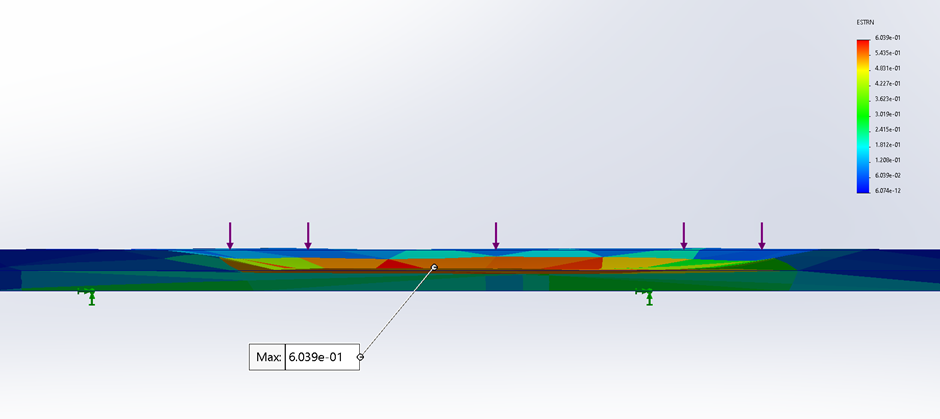
\includegraphics[width=0.6\linewidth]{Figures/d13mm_20N_load_ESTRN_max_FEM.png}
	% \includegraphics[width=0.35\linewidth]{Figures/d13mm_20N_load_ESTRN_max_FEM_3d.png}
	% \caption{Strain mesh of 13 mm diameter 20 N load case FEM model. Left: Cross-section. Right: 3D view.}
	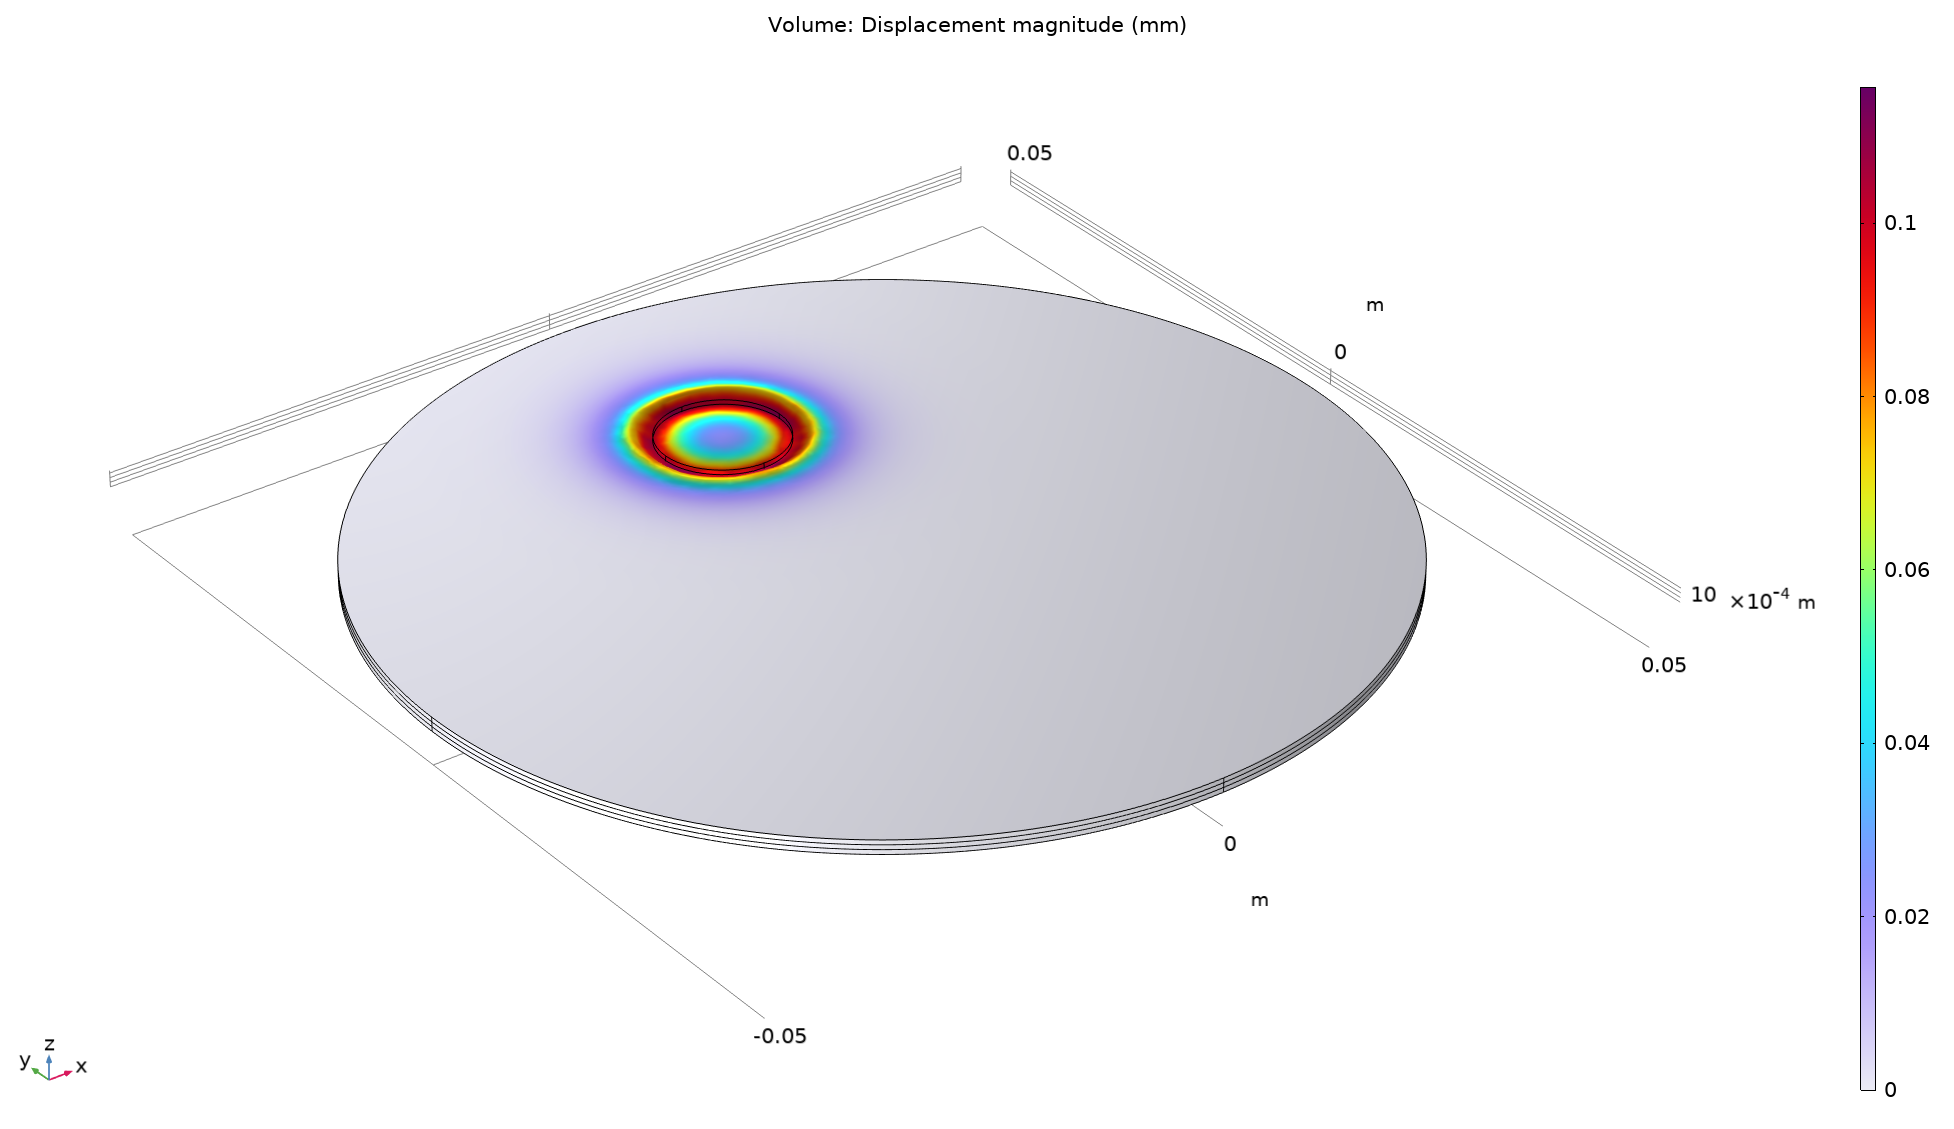
\includegraphics[width=0.7\linewidth]{Figures/d13mm_load_3d_disp.png}
	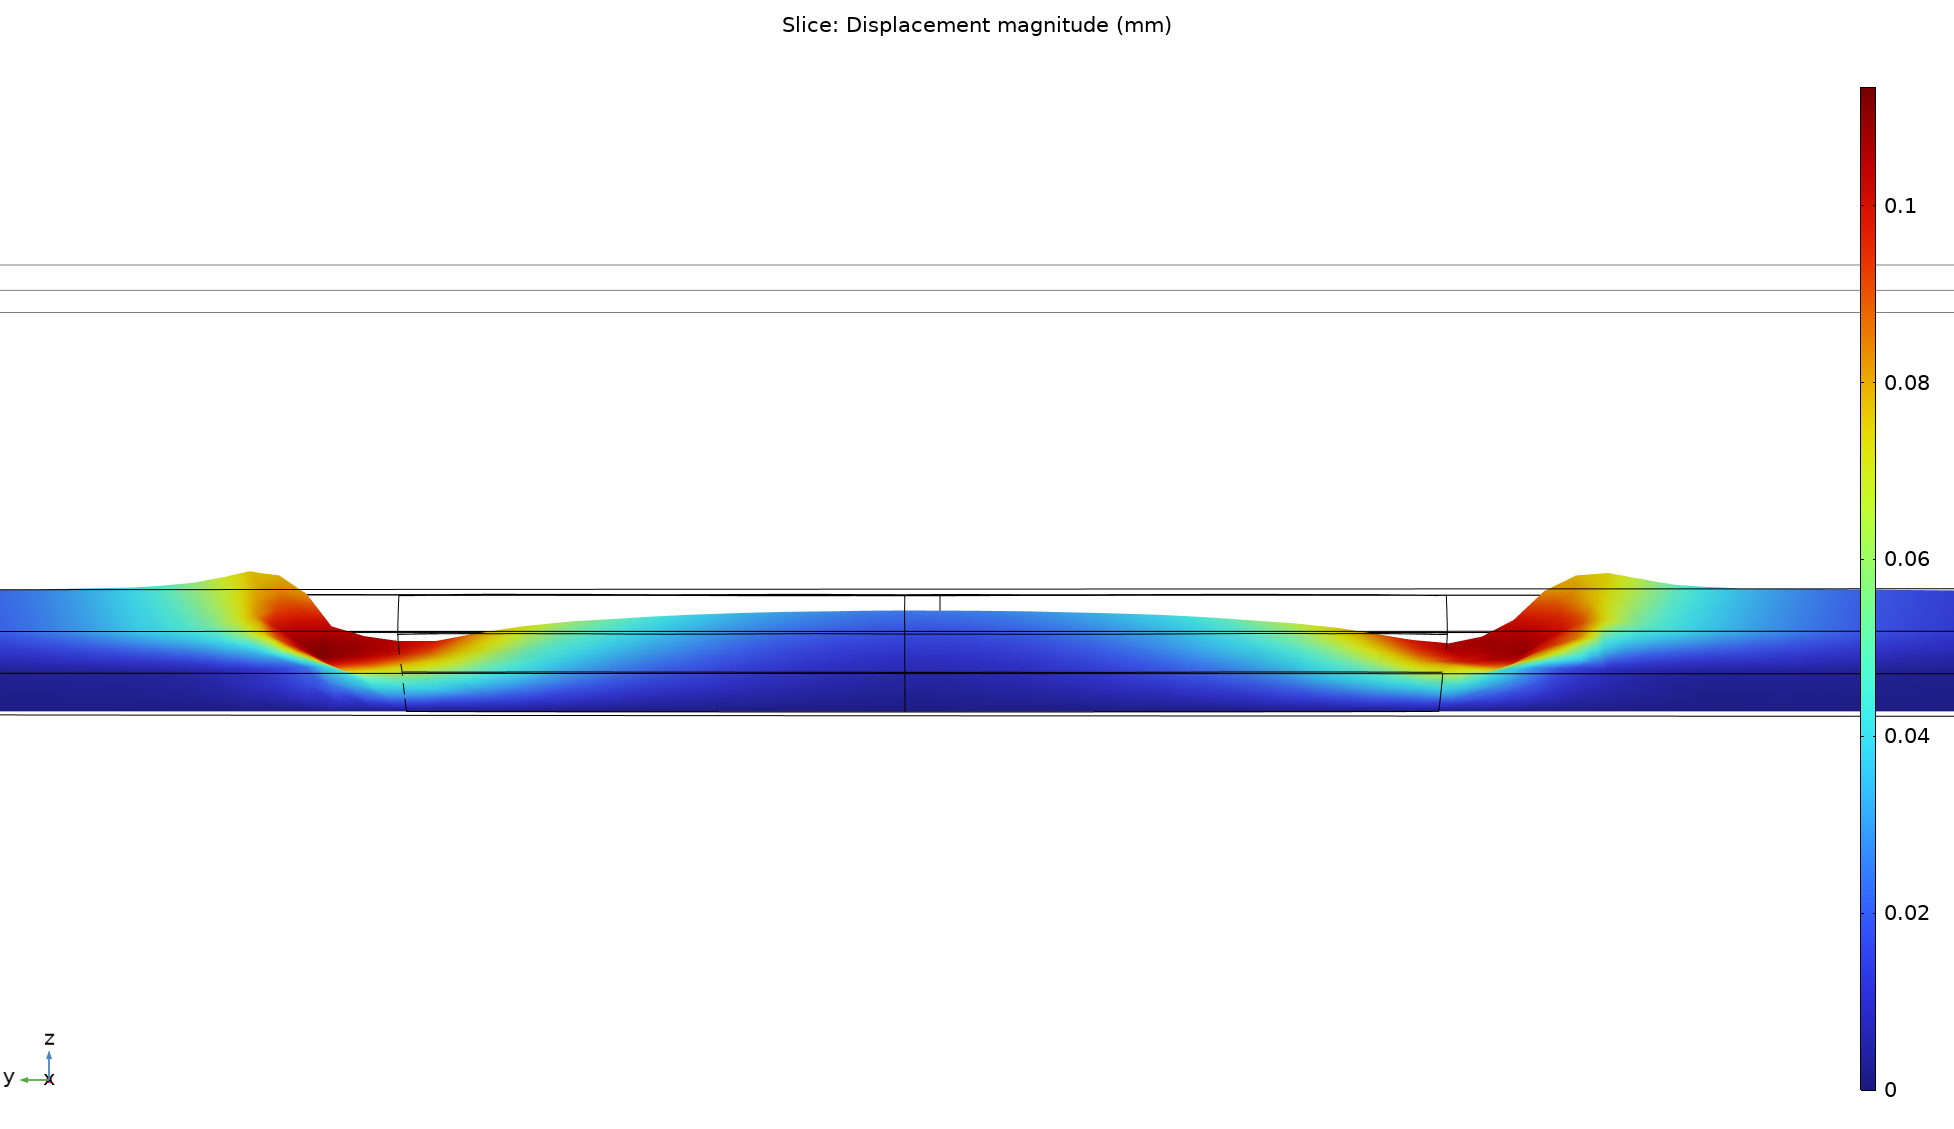
\includegraphics[width=0.7\linewidth]{Figures/d13mm_load_zoom.png}
	\caption{Deformed mesh plot of 13 mm diameter 20 N load case FEM model (x10 scale displacement). Top: 3D view. Bottom: Cross-section zoomed view.}
	\label{fig:FEM_DEA-EIT_loading}
\end{figure}


\subsection{Deformed DEA Electrostatics Study}
The deformed DEA-EIT structure causes the overall capacitance across the device electrodes to increase. The first step was running an electrostatic FEM study to generate an electric field, as shown in Figure \ref{fig:FEM_DEA-EIT_cap}.
%% Todo: FEM electric field plot example (redo!!)
%% Todo: re-run with a higher voltage or having a logarithmic scale for electric field lines
\begin{figure}[H]
	\centering
	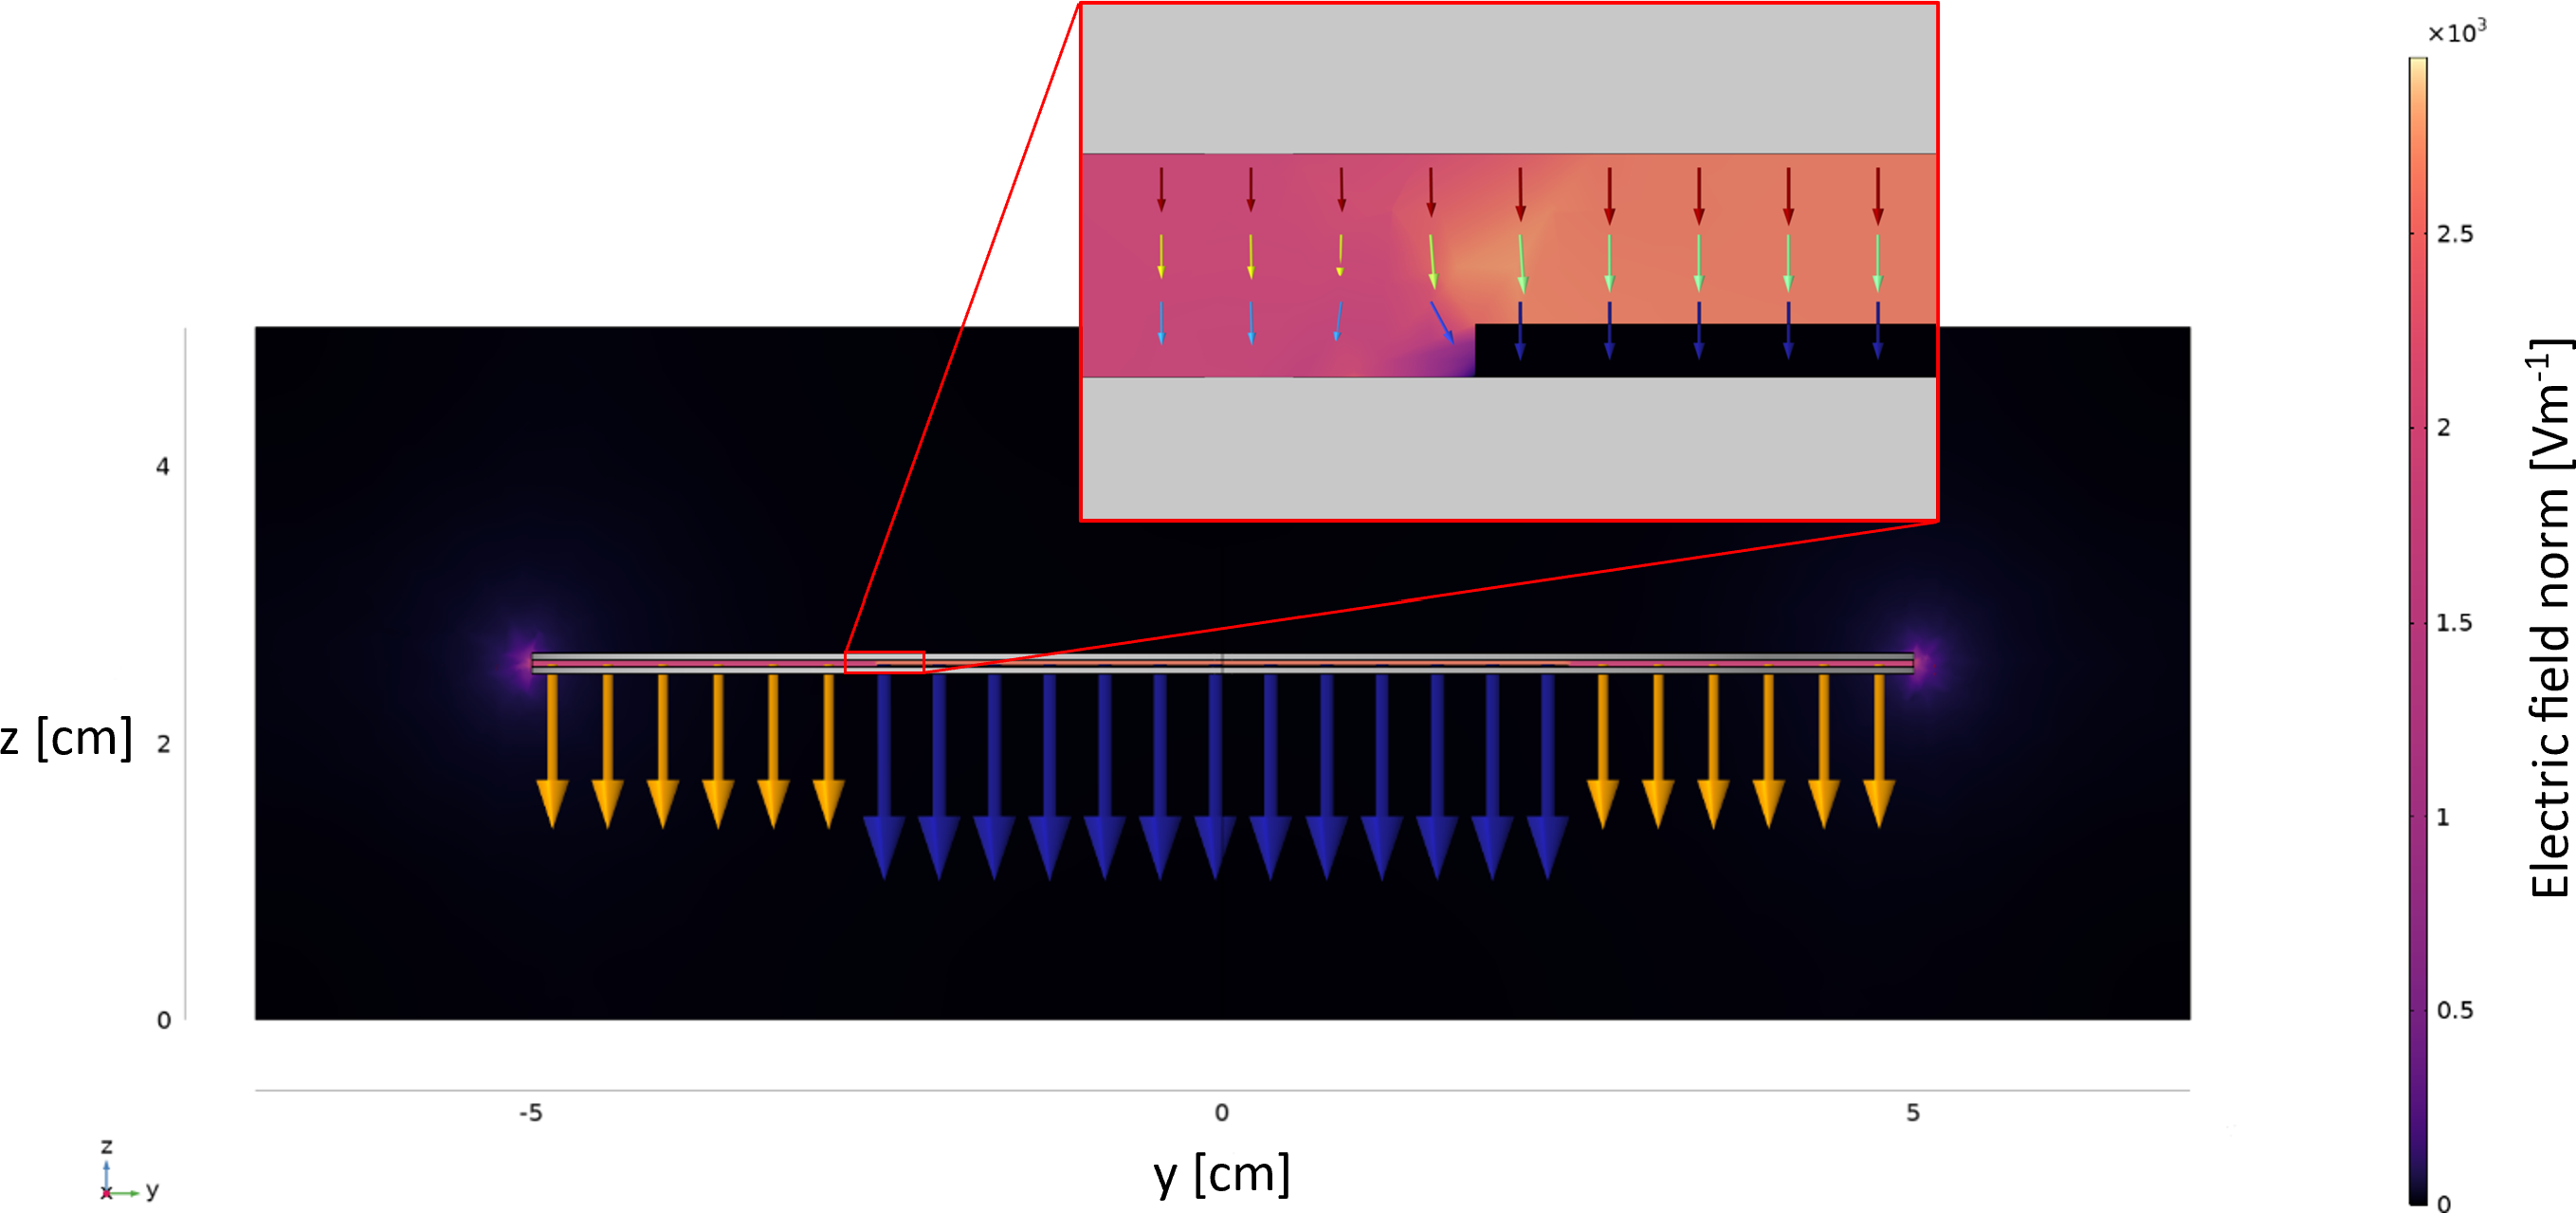
\includegraphics[width=\linewidth]{Figures/d50mm_load_labelled_shoulder_zoom.png}
	\caption{Electric field simulation of 50 mm diameter 240 N load case. With a zoomed section to show the electric field `fringe' effects at the shoulder of the load cross-section. Volumetric arrows proportional to electric field strength.}
	\label{fig:FEM_DEA-EIT_cap}
\end{figure}


\subsection{Voltage and Energy Generation}
\label{subsec:Voltage and Energy Generation}
To show the scale at which energy is generated an example scenario for the extra voltage generated is given. Given that the values from Figure \ref{fig:dea_eit_deg} are, $C_i = 10 pF$, $C_{ii} = 15 pF$, and $V_i = 5 kV$. We get a charge $Q = 75 nC$, and then at stage D, $V_{ii} = \frac{Q}{C_{i}} = 7.5 kV$. This gives a voltage change, $\Delta V = +2.5 kV$.

The parallel plate assumption for calculating capacitance of the DEA-EIT becomes invalid for the deformed DEA-EIT device. An approximation utilising the electric field FEM result on the deformed DEA-EIT FEM result is calculated using Maxwell capacitance matrix.

The change in capacitance was used to calculate the generated energy and voltage, values from the experiment are shown in Tables \ref{tab:volt-energy-gen-d13mm} and \ref{tab:volt-energy-gen-50mm}.

%% Todo: Add energy generated column for each case
\begin{table}[H]
	\centering
	\caption{Voltage and energy generation results calculated from FEM values for the 13 mm diameter load cases.}
	\label{tab:volt-energy-gen-d13mm}
	\vspace{0.3cm}
	\begin{tabular}{llllll}
		\textbf{Load [N]} & \textbf{ESTRN} & \textbf{C [pF]} & \textbf{dC [pF]} & \textbf{dV$_{DE}$ [V]} & \textbf{dU [uJ]} \\ \hline
		0.00  & 0.00 & 588.86 & 0.00  & 0.00   & 0.00    \\
		2.50  & 0.08 & 589.69 & 0.83  & 7.04   & 31.14   \\
		5.00  & 0.15 & 590.73 & 1.87  & 15.83  & 70.20   \\
		10.00 & 0.30 & 593.40 & 4.54  & 38.25  & 170.68  \\
		20.00 & 0.60 & 605.53 & 16.67 & 137.65 & 630.86  \\
		30.00 & 0.91 & 688.18 & 99.32 & 721.61 & 3903.68
	\end{tabular}
\end{table}

%% Todo: Add energy generated column for each case
\begin{table}[H]
	\centering
	\caption{Voltage and energy generation results calculated from FEM values for the 50 mm diameter load cases.}
	\label{tab:volt-energy-gen-50mm}
	\vspace{0.3cm}
	\begin{tabular}{llllll}
		\textbf{Load [N]} & \textbf{ESTRN} & \textbf{C [pF]} & \textbf{dC [pF]} & \textbf{dV$_{DE}$ [V]} & \textbf{dU [uJ]} \\ \hline
		0.00 & 0.00 & 588.86 & 0.00 & 0.00 & 0.00 \\
		% 5.00 & 0.01 & mesh   error - too fine & \#VALUE! & \#VALUE! & \#VALUE! \\
		10.00 & 0.02 & 591.90 & 3.04 & 25.68 & 0.20 \\
		20.00 & 0.04 & 595.00 & 6.14 & 51.60 & 0.79 \\
		30.00 & 0.06 & 598.33 & 9.47 & 79.14 & 1.87 \\
		60.00 & 0.12 & 609.24 & 20.38 & 167.26 & 8.52 \\
		120.00 & 0.24 & 635.86 & 47.00 & 369.58 & 43.43 \\
		240.00 & 0.48 & 727.10 & 138.24 & 950.63 & 328.54
	\end{tabular}
\end{table}

To validate the capacitance results form Tables \ref{tab:volt-energy-gen-d13mm} and \ref{tab:volt-energy-gen-50mm} the the capacitance was solved analytically using the parallel-plate capacitance approximation given in Equation \ref{eqn:capacitance}. Matching the parameters of the FEA simulation the capacitance of the 100 mm DEA device with no load applied, the capacitance was approximated to be 584.13 pF.

A comparison of two similar trends for different loads applied to the DEG using FEM and an analytical method can be observed in Figure \ref{fig:volt-energy-gen-13_and_50mm}. The analytical solution is given in Appendix \ref{appendix-F}.

\begin{figure}[H]
	\centering
	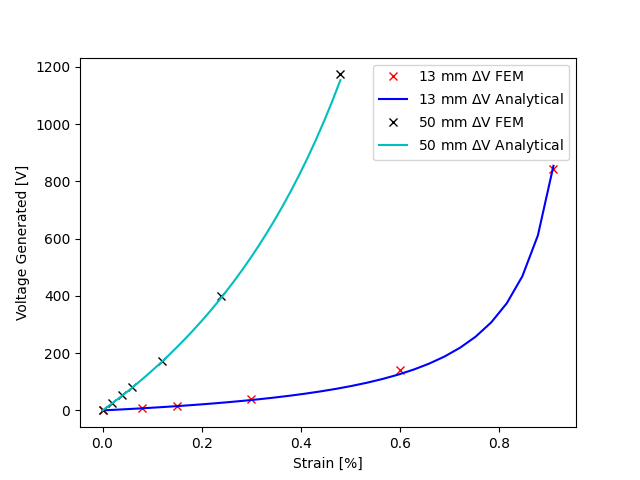
\includegraphics[width=0.65\linewidth]{Figures/plot_DEG_strain_vs_Vgen_FEM_vs_analytical.png}
	\caption{FEM vs analytical solution for voltage generation, $\Delta V$, for an initial voltage input of 5 kV for the range of loads applied.}
	\label{fig:volt-energy-gen-13_and_50mm}
\end{figure}


\section{Discussion}
\label{sec:discussion}
% Small impact statement!
The results from this work show promise towards understanding the energy generated from an EIT-DEA device when used in a particular fashion. The FEA simulations completed were validated analytically with a small discrepancy of 4.73 pF, i.e. 0.8\% error, due to the electric field fringe effects the parallel plate capacitor assumption does not account for. The plot shown in Figure \ref{fig:volt-energy-gen-13_and_50mm} shows the trends for a 13 mm and 50 mm load applicator, from this decreasing the dielectric thickness is seen to give a large increase in voltage and energy generated. At these high strains the likelihood of dielectric break through is significantly increased, especially so in a real world scenario when the load surface may contain sharp features, piercing or forming stress concentrations within the DE. The comparison of the FEM and analytical approximation in Figure \ref{fig:volt-energy-gen-13_and_50mm_err} shows that the fringing electric field effect increases with increasing input strain deformation.

\begin{figure}[H]
	\centering
	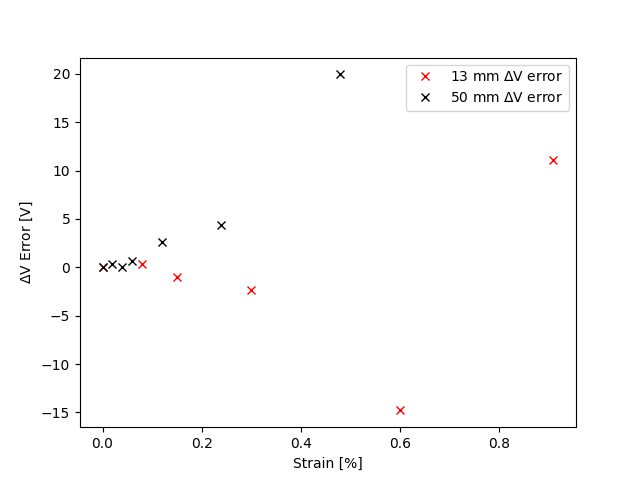
\includegraphics[width=0.65\linewidth]{Figures/plot_DEG_strain_vs_Vgen_err.png}
	\caption{FEM vs analytical solution error for voltage generation, $\Delta V$, for an initial voltage input of 5 kV for the range of loads applied.}
	\label{fig:volt-energy-gen-13_and_50mm_err}
\end{figure}

% useful applications
% how to harness it
The energy generated by the sequence shown in Figure \ref{fig:dea_eit_deg}, can be harnessed if there is a sensing mechanism put in place to determine when the capacitance of the DEA will change and apply the voltage appropriately. Conversely, this energy generation can be undesirable for certain applications as it may cause damage to the attached circuitry.

Such energy generation case may be avoided in a system by detecting that a pressure event has occurred and preventing the excitation of the DEA or limiting the charge accumulation on each plate of the capacitor. Example applications could include a DEA-EIT device laid on a surface such as a road or footpath for surveying and energy generation from vehicular or foot traffic loads.

An example scenario of voltage and energy generation was given in Section \ref{subsec:Voltage and Energy Generation}. This voltage change transient could be connected to an EIT multiplexer through the capacitance of the DEA, as shown by Equation \ref{eqn:mux_voltage}. The multiplexer pins used in this case are limited to between the power rails, i.e. $\pm$22 V \cite{VishayPG2018}. In the case described above the minute change in capacitance of the DEA is calculated to generate 93.75 $\mu$J of energy.

To determine the device's tolerance against transient voltage spikes, the EIT multiplexer limits would need to be characterised. Otherwise, in the case of an input pin overvoltage CMOS latch-up may occur \cite{Redmond2001} . Typical ESD standards \cite{IEC2008} state that electronic devices must be tolerant to 200 pF capacitance charged to $\pm$15 kV, giving an energy dissipation of 22.5 mJ. This is several orders of magnitude larger than the energy generated in the simulation results shown in Tables \ref{tab:volt-energy-gen-d13mm} and \ref{tab:volt-energy-gen-50mm}. However, for different configurations of DEA device this energy generation may become significant.
%% justify above statement with references. I.e. how much energy is in a standardised maximum ESD discharge. Typical ESD devices have a 100-200 pF capacitance charged up to 8 - 15 kV voltage. 



% To do: Address idealness of FEM study completed and how physical experimentation could help create a relationship between the simulated and real data in future.
% To do: Run some experiments to see roughly if the same trend from the simulated data is seen in real-life.

\section{Conclusions}
% Overall conclusion ... Can be prevented, only significant if delta C is large, requires more testing, could create a DEG-EIT device to capture data from cars, foot traffic?

This work has investigated the prominence of energy generation of a 100 mm diameter DEA device with a 500 $\mu$m dielectric elastomer. The sequence by which this energy generation occurs has been explained, and several scenarios have been tested for energy generation from localised 13 mm and 50 mm diameter loads with magnitudes ranging from 0 - 240 N. Depending on the load force, 0.2 $\mu$J to 4 mJ of energy generation has been estimated. Although these are small energy values, often DEAs require large voltages to actuate so any amplification of these voltages needs to be handled on a case by case basis for each application and DEA device. Using methods to estimate the occurrence of a change in DEA capacitance is recommended in all applications to either avoid or harness this energy generation. Potential future applications of a device that utilises this energy generation ranges from vehicular traffic loads to foot traffic loads. Future work aims to to validate the simulated findings and determine the energy losses in a real world application. Then in further future work the designed DEG system may be created and used to power a EIT-based pressure sensing circuit. 

%\afterpage{\blankpage}